

% !TeX encoding = UTF-8
% !TeX spellcheck = de\\_DE

%% Dies gibt Warnungen aus, sollten veraltete LaTeX-Befehle verwendet werden
\RequirePackage[l2tabu, orthodox]{nag}
\documentclass[utf8,biblatex, ngerman, english]{lni}
\usepackage{url}
\bibliography{literatur.bib}


%% Schöne Tabellen mittels \toprule, \midrule, \bottomrule
\usepackage{booktabs}

%% Zu Demonstrationszwecken
\usepackage[math]{blindtext}
\usepackage{mwe}

 

%% BibLaTeX-Sonderkonfiguration,
%% falls man schnell eine existierende Bibliographie wiederverwenden will, aber nicht die .bib-Datei händisch anpassen möchte.
%% Bitte \iffalse und \fi entfernen, dann ist diese Konfiguration aktiviert.

\iffalse
\AtEveryBibitem{%
  \ifentrytype{article}{%
  }{%
    \clearfield{doi}%
    \clearfield{issn}%
    \clearfield{url}%
    \clearfield{urldate}%
  }%
  \ifentrytype{inproceedings}{%
  }{%
    \clearfield{doi}%
    \clearfield{issn}%
    \clearfield{url}%
    \clearfield{urldate}%
  }%
}
\fi

\begin{document}

%%% Mehrere Autoren werden durch \and voneinander getrennt.
%%% Die Fußnote enthält die Adresse sowie eine E-Mail-Adresse.
%%% Das optionale Argument (sofern angegeben) wird für die Kopfzeile verwendet.
\title[WSL]{Windows Subsystem for Linux}
%%%\subtitle{Untertitel / Subtitle} % falls benötigt
\author[Marius Rusu \and Julia Sommer]
{Marius Rusu\footnote{Ludwig-Maximilian-Universität München, Fakultät für Informatik, Oettingenstraße 67, 80538 München, Deutschland \email{rusu.marius97@gmail.com}} \and
 Julia Sommer\footnote{Technische Universität München, Fakultät für Informatik, Boltzmanstraße 3, 85748 Garching, Deutschland \email{sommerjulia99@gmail.com}}}
\editor{Herausgeber et al.}    % Namen der Herausgeber
\booktitle{Name-der-Konferenz} % Name des Tagungsband
\year{2017}
%%%\lnidoi{18.18420/provided-by-editor-02} % Falls bekannt
\maketitle
\newpage
\tableofcontents
\newpage

\begin{abstract}
The Windows Subsystem for Linux is a new feature that enables running native Linux command-line tools directly on Windows. This paper shall investigate its architecture and implementation and compare it to other common Linux virtualizations.
\end{abstract}

\begin{keywords}
Windows Subsystem for Linux \and Virtualization
\end{keywords}

\section{Microsoft's reasons for WSL}

Many programmers that work with open source, Linux based tools such as Pearl and Python are struggeling on Windows. Especially when it comes to server infrastructure, programmers work with applications native to Linux since most of the Servers are also powered by Linux. Those applications unsually do not work great on Windows and programmers depend on workarounds like Containers and Virtual Machines. Alternatively, they switch to Linux or other Unix based operating systems \cite{Ha16c}.

Based on their feedback, Microsoft made investments that improve cmd, PowerShell and many other command-line tools and developer scenarios. According to Mike Harsh, they further decided to grow their command line family by adding real, native Bash and with it support for Linux command-line tools which run directly on Windows in an environment that behaves like Linux.
To accomplish this, Microsoft worked together with Cononical and published the Windows Subsystem for Linux running Ubuntu in April 2016\cite{Ha16c}.


\section{Windows Subsystem for Linux}
The following will provide information about the Windows Subsystem for Linux, based on Microsoft's publication.

\subsection{General Concept}
"Windows Subsystem for Linux is a collection of [user mode and kernel mode] components that enable native Linux ELF64 binaries to run on Windows \cite{Ha16b}."\ User mode applications are low privileged and depend on system calls to operate on kernel mode. Only in kernel mode low level operations directly handled by the operating system can be executed. In WSL we have the bash.exe running in user mode and initiating the Linux Instance. Further this instance submits, if necessary, native Linux system calls to be executed on a Linux Kernel. However, by virtualizing a Linux Kernel interface those system calls can be executed directly on the Windows Kernel. This virtualization is done by the LXCore/LXSS running in kernel mode \cite{Ha16b}.

\subsection{Basic Architecture}



Windows Subsystem for Linux "\ is primarily comprised of: 
\begin{enumerate}
    \item LX Session Manager
    \item LXCore/LXSS
    \item Pico processes
\end{enumerate}\cite{Ha16b}"

\begin{figure}
  \centering
  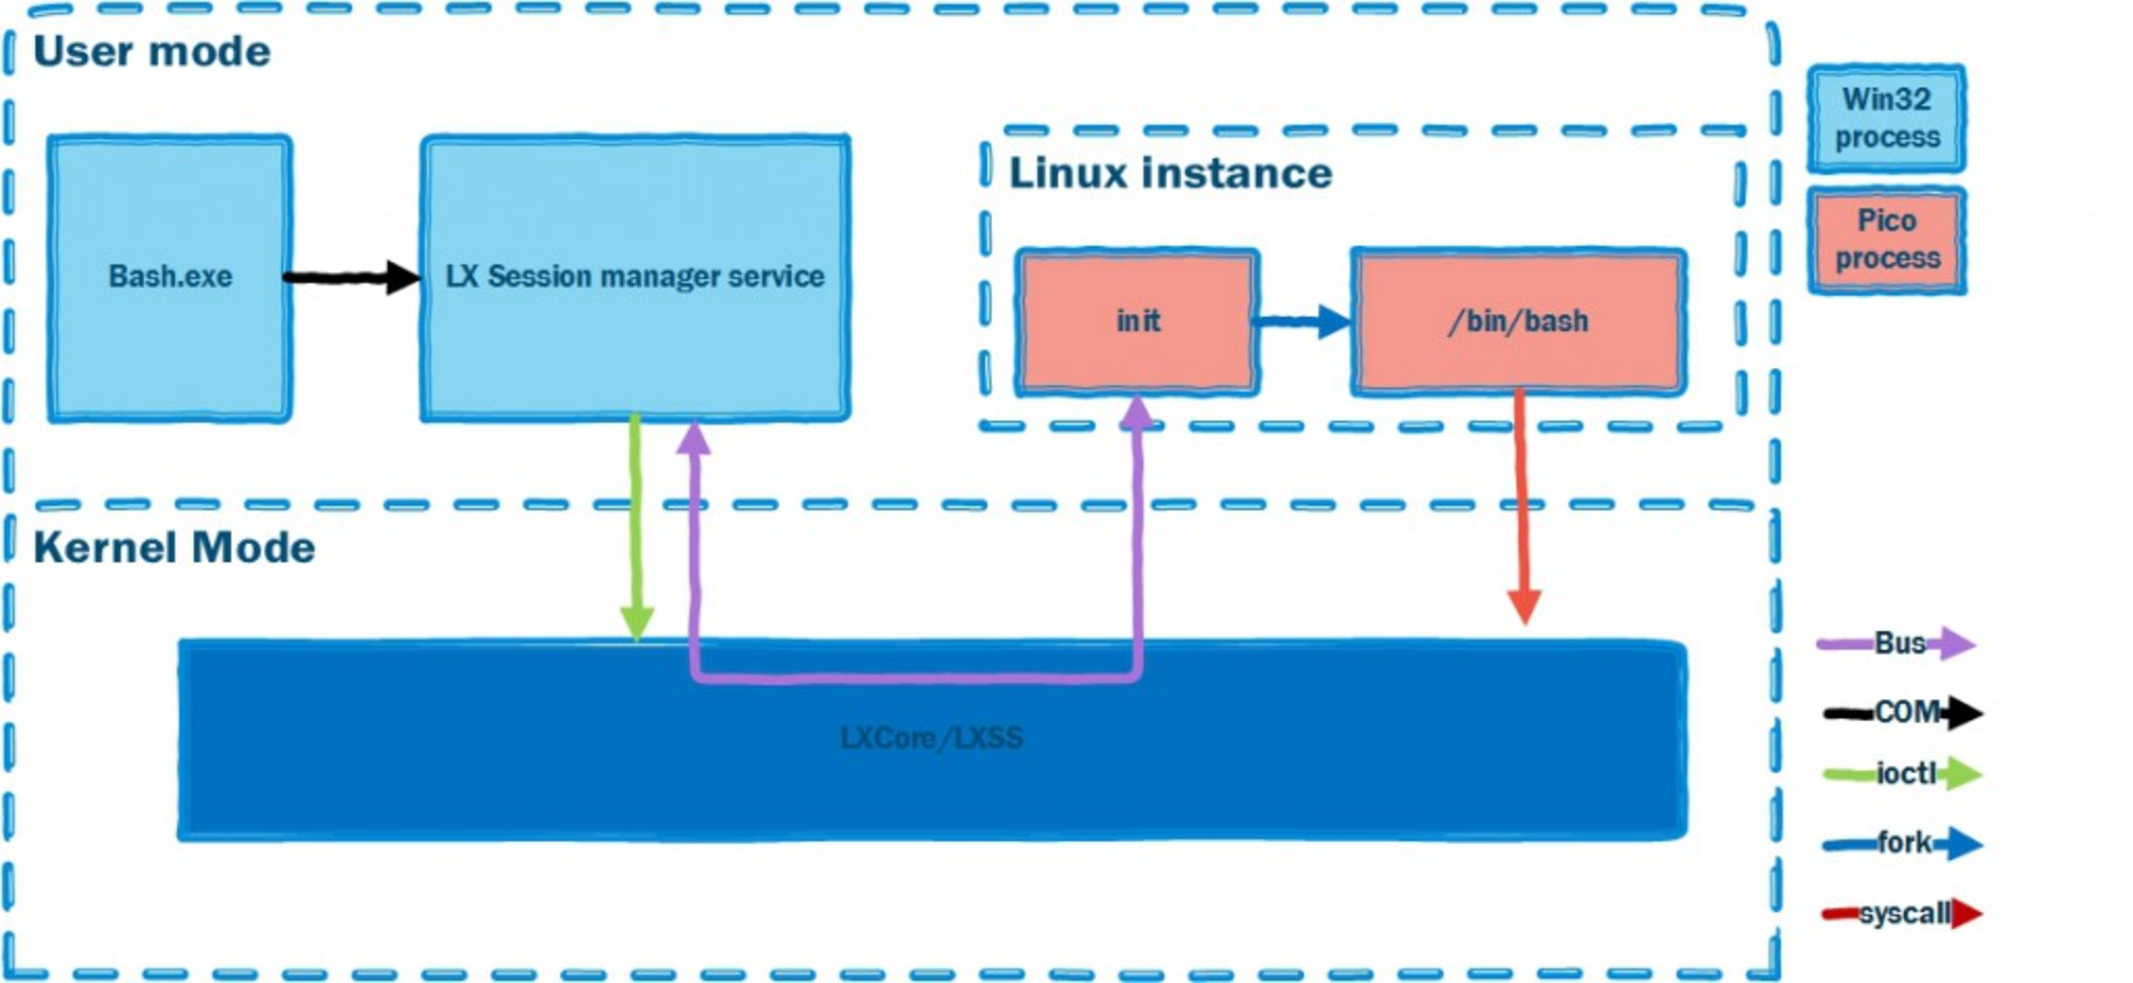
\includegraphics[width=1\textwidth]{WSL Architecture.pdf}
  \caption{Main components of WSL \cite{Ha16b}}
  \label{img:architecture}
\end{figure}

As depicted in the image above \ref{img:architecture}, the user initiates the Windows Subsystem for Linux by launching the bash.exe on Windows. According to Nick Judge, this application then calls the LXCore/LXSS (green arrow) which is a driver behaving like a Linux Kernel and working in coordination with the Windows Kernel. The Driver would then spin up a native Linux process being /bin/bash (purple arrow). All other Linux processes run under /bin/bash in the so called Linux Instance that you can think of as a container or a virtualized operating system environment \cite{Ha16a}."

"By wrapping unmodified Linux binaries into pico processes we enable Linux system calls to be directed into the Windows kernel \cite{Ha16b}."\ A pico process itself is an empty process, as far as the Windows kernel is concerned and therefore cannot be handled by the Windows kernel but instead is redirected to the LXCore/LXSS (red arrow) \cite{Ha16a}.
Therefore "pico processes and drivers [LXCore/LXSS] provide the foundation for the Windows Subsystem for Linux\cite{Ha16b}."

\subsection{Implementation of its components}

"The pico process concept originated in MSR [Microsoft Research] as part of the Drawbridge project. A goal of this project was to implement a lightweight way to run an application in an isolated environment, with the application’s OS dependencies decoupled from the underlying host OS \cite{Ha16a}."\ This was achieved, not by a Virtual machine, which would be too resource consuming but by "run[ning] the target application and OS entirely within the usermode address space of a single process on the host OS \cite{Ha16a}". The Drawbridge pico process is a lightweight, secure isolation container. It is built from an OS process address space, but with all traditional OS services removed. "\ All ABI [Application binary interface] calls are serviced by the security monitor, which plays a role similar to the hypervisor or VM monitor in traditional hardware VM designs \cite{11}."

In case of Windows subsystem for Linux this is exactly the point where pico processes are redirected to the LXCore/LXSS. "The drivers do not contain code from the Linux kernel but are instead a clean room implementation of Linux-compatible kernel interfaces. [..] Where possible, lxcore.sys translates the Linux syscall to the equivalent Windows NT call which in turn does the heavy lifting. Where there is no reasonable mapping the Windows kernel mode driver must service the request directly \cite{Ha16b}."\ Since the Windows Kernel was originally designed to support multiple operating systems, Microsoft had to dust of old functionality, enhance it for performance and correctness and it was able to go right away, says Nick Judge \cite{Ha16a}. Those changes in the Windows kernel enable it to execute even foreign operations like fork(). Windows applications however do not have access to those specific Linux system calls.

"The File system support in WSL was designed to meet two goals:
\begin{enumerate}
    \item Provide an environment that supports the full fidelity of Linux file systems
    \item Allow interoperability with drives and files in Windows 
\end{enumerate}\cite{Ha16b}"

"VolFs is a file system that provides full support for Linux file system features, including Linux permissions that can be modified through operations such as chmod and chroot [...]\cite{Ha16b}"\ and other features. Due to the fact that VolFs file system is not able to interoperate with Windows, a second file system named DriveFs is implemented. "\ All fixed Windows volumes are mounted under /mnt/c, /mnt/d, etc. [...]. This is where users can access all Windows files\cite{Ha16b}."\ To make this possible the DriveFs file system meets Windows requirements such as legal file names and Windows security but looses some of the Linux features.

\section{Alternatives to Windows Subsystem for Linux}
The following will discuss other possibilities of running Linux on Windows and compare them to the Windows Subsystem for Linux.

\subsection{Virtualization via Virtual Machine}

\begin{figure}
  \centering
  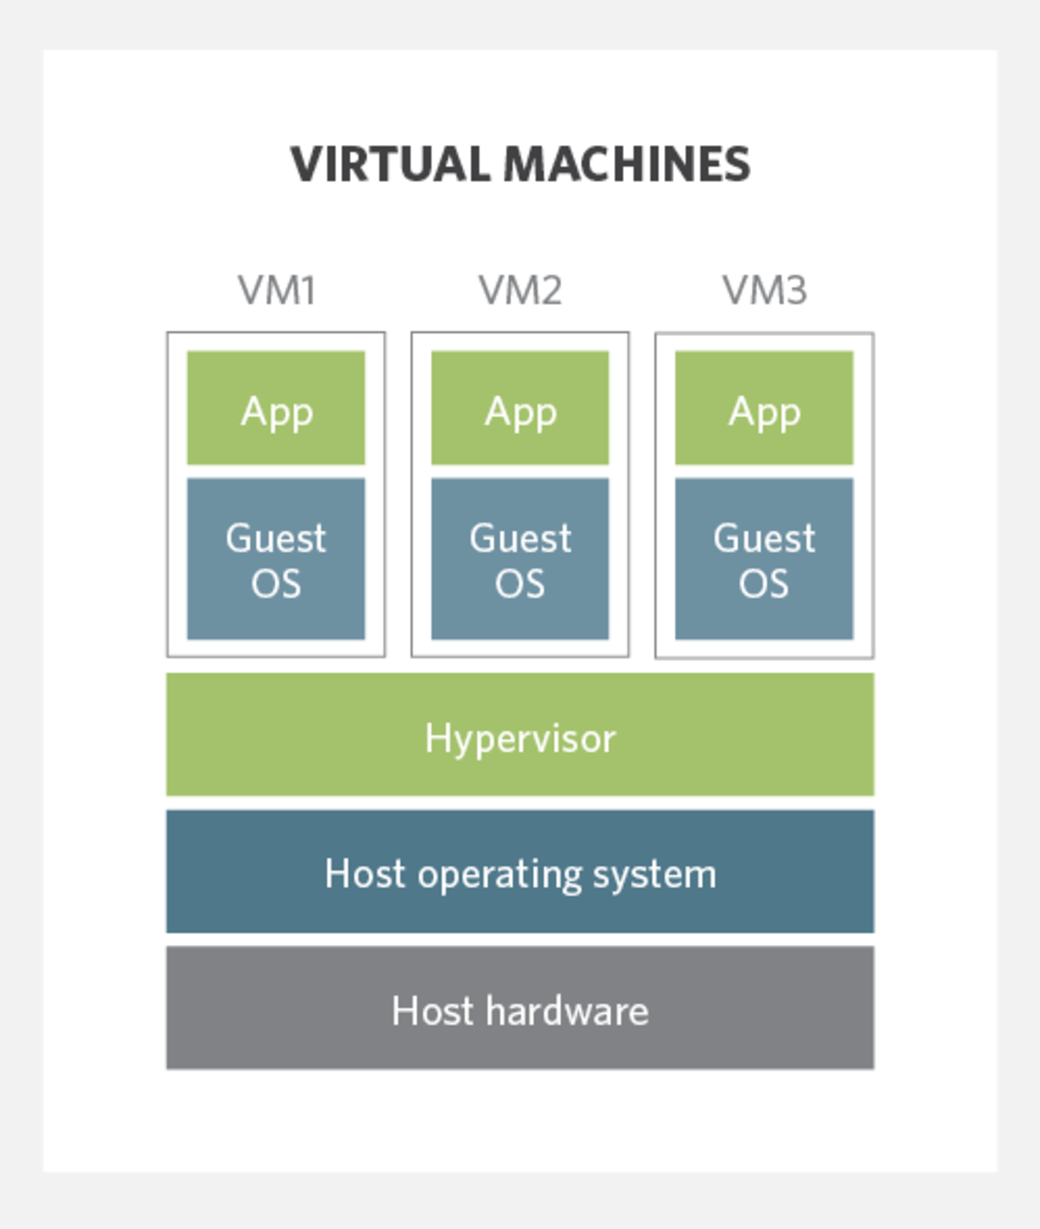
\includegraphics[width=0.5\textwidth]{VM.pdf}
  \caption{Virtual Machine Overview}
  \label{img:vm}
\end{figure}


"The virtual machine concept allows the same computer to be shared as if it were several. IBM [(International Business Machines Corporation)] defined the virtual machine as a fully protected and isolated copy of the underlying physical machine’s hardware \cite[p. 2]{Ro01}."\ 
Therefore it is possible to run different applications on different operating systems at the same time on the same hardware as depicted in the image above. "The VMM [(Virtual Machine Monitor)] is the software component that hosts guest virtual machines \cite[p. 3]{Ro01}." \ \ The Virtual Machine Monitor is firstly responsible for coordinating the access of the guest operation systems on the host's hardware and secondly for handling traps. Traps are created when a guest operating system is trying to execute a privileged operation. In that case, the Virtual Machine Monitor emulates its function in order to be executed on the host operating system.

\begin{figure}
  \centering
  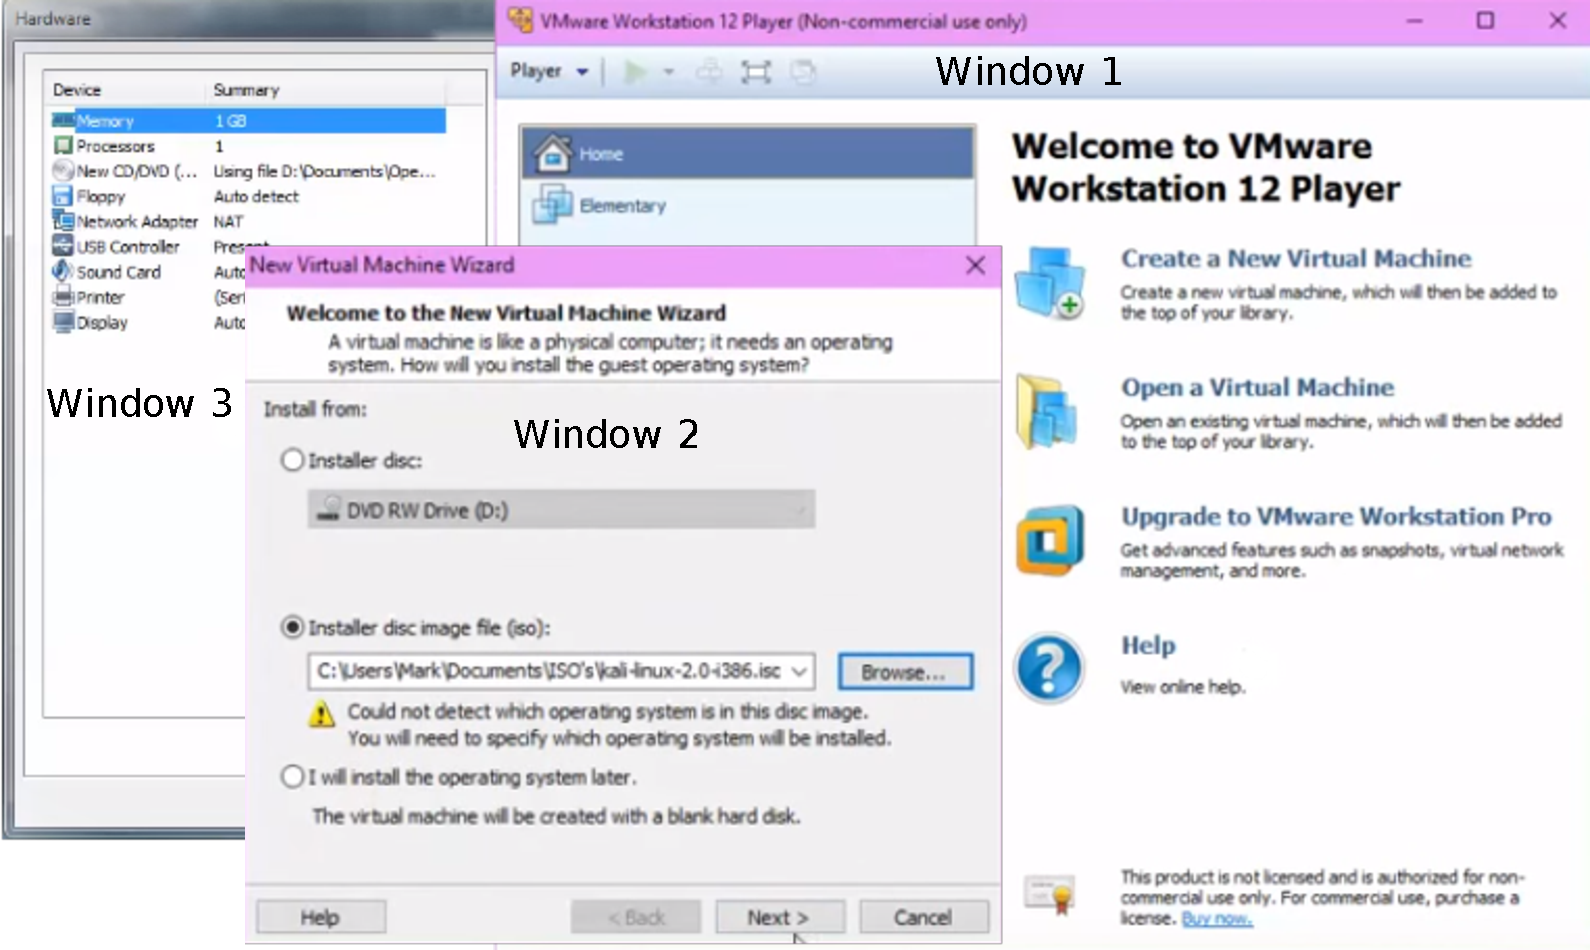
\includegraphics[width=0.9\textwidth]{VMware Player.pdf}
  \caption{VMware Player's graphic interface}
  \label{img:VMwarePlayer}
\end{figure}

A common tool for creating a virtual machine is VMware Player by VMware Inc. This application hides all the work of the Virtual Machine Monitor and comes with a graphic interface that can be seen above (Window 1)\ \ref{img:VMwarePlayer}. For creating a new virtual machine an image file of the guest operating system is needed, which can be either on a disc or downloaded from the internet (Window 2)\ \ref{img:VMwarePlayer}. After this, the user can decide on how many ressources, e.g. memory space and CPU cores the new virtual machine can use (Window 3)\ \ref{img:VMwarePlayer}. Finally, VMware Player launches the guest operating system in a new window as a fully functional and isolated operating system.

\subsection{Virtualization via Container}

\begin{figure}
  \centering
  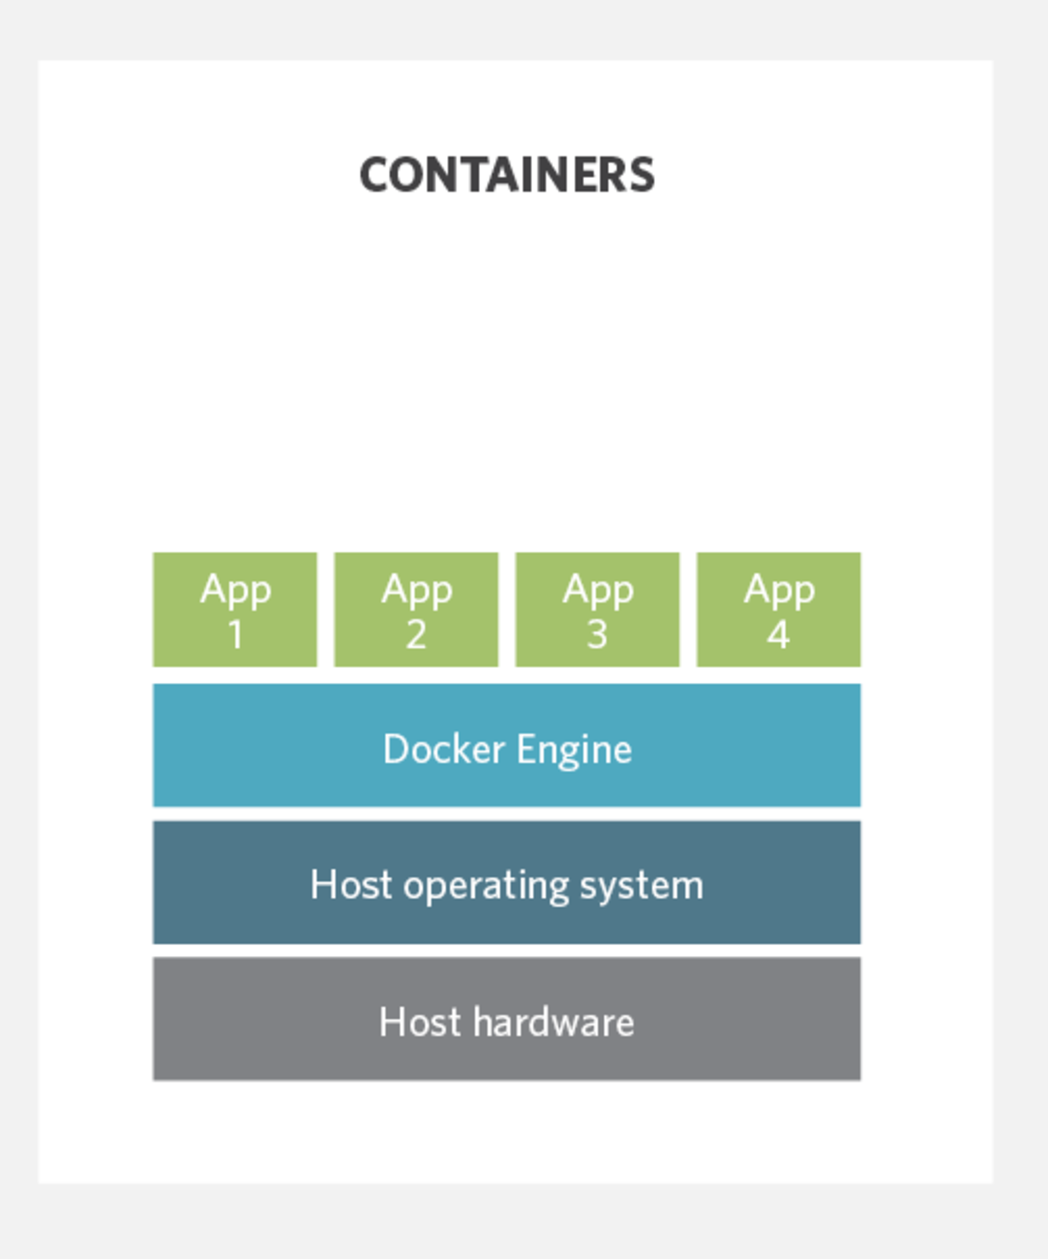
\includegraphics[width=0.5\textwidth]{Container.pdf}
  \caption{Container Overview}
  \label{img:container}
\end{figure}

Rather than virtualizing the hardware, containers use the host operating system and share its kernel. According to V. Badola containers are "\ stripped down Virtual Machines running just enough software to deploy an application \cite{Ba15}."\ \ Instead of a Virtual Machine Monitor there is a container engine running on top on the host operating system which can be seen in the image below \ref{img:container}. "\ A container engine is a managed environment for deploying containerized applications. The container engine allocates cores and memory to containers [and] enforces spatial isolation and security [...] \cite{Do17}."

One of the most used container engines is the open source Docker, which developed a method to give containers better portability. According to Margaret Rouse "with Docker containers, there are no guest OS environment variables or library dependencies to manage \cite{Ma}."\ In order to run a container in Docker, a so called Dockerfile is needed. "Dockerfile instructions provide the Docker Engine with the steps needed to create a container image \cite{La16}."\ Dockerfiles contain firstly the image of the system environment of the container, secondly the application to run and thirdly the port for communication between host and container. Docker Hub provides users with a collection of images e.g. Ubuntu for download. All those steps are done in the console and a text editor for the Dockerfile, since there is no graphic interface.

\subsection{Comparison to Windows Subsystem for Linux}

In view of all the facts, Windows Subsystem for Linux is neither a Virtual Machine nor a Container but rather something in between. Is not a fully virtualized Linux operating system which would be the result of a Virtual Machine but is also more than just a Container environment. There are three major differences that result in advantage and disadvantages. 

First of all Windows Subsystem for Linux is not isolated from the host operating system but rather works hand in hand. This can be seen by the fact that processes are directly handled by the host kernel instead of a Virtual Machine Monitor or Container Engine. Further, the file systems VolFs and DriveFs are both accessible from Windows and Linux while Containers and Virtual Machines are usually invisible to each other. This can be a disadvantage especially when running possibly dangerous or unstable programms. While there are security measures, there have been fears that malware can reach Windows via the Linux Subsystem. \cite{Tu17}. It can also be an advantage for the common user that wants to access and edit Windows files with open source, Linux native tools or want to run their programms on both operating systems for debugging without having to launch a Virtual Machine or Container.

Secondly, there exists only one Linux instance for each user. All programms run together under /bin/bash and cannot be separated from each other. Even launching Ubuntu more than once will always result in thae same Linux instance\cite{Ha16b}. This is a disadvantage if an isolated environment is needed. This case is similar to the security concerns between Windows und the Linux Subsystem mentioned above but this time it affects programms inside the Linux Instance. In both cases a fully isolated Virtual Machine or 
Container is the better choice.

\begin{figure}
  \centering
  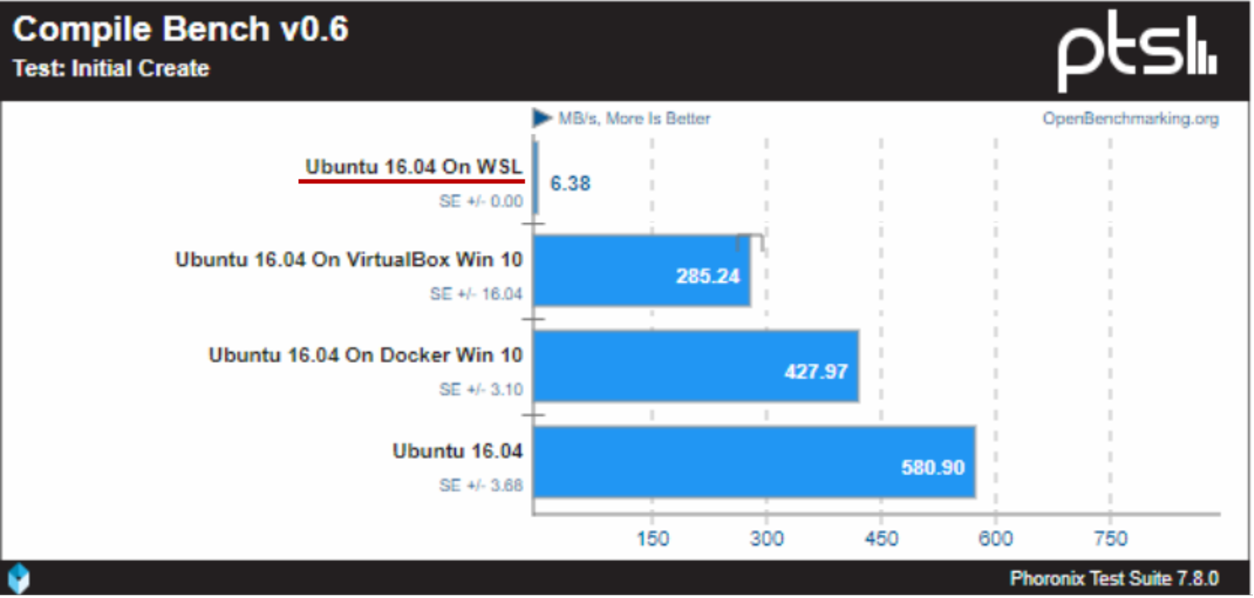
\includegraphics[width=0.8\textwidth]{CompileSpeed.pdf}
  \caption{Compile Benchmark}\cite{La18} 
  \label{img:speed}
\end{figure}

Thirdly, there are differences regarding the performance of those three attemps of virtualization. According to tests run by Phoronix, the I/O performance of the Windows Subsystem for Linux rather laggs behind as can be seen in the image above \ref{img:speed}. This issue has even become worse since the Spectre/Meltdown updates, which were supposed to mitigate those security vulnerabilities. "\ If exploited, these vulnerabilities can give hackers unprecedented access to compromised systems and widespread liberty to steal a broad variety of confidential, sensitive data \cite{Pe18}."\ The poor I/O performance is certainly the biggest disadvantage of the Windows Subsystem for Linux and the reason it cannot fully replace Virtual Machines or Containers yet. On the other hand, Windows Subsystem for Linux performs at least as good as Virtual Machines and Containers when it comes to MP3/FFMPEG encoding and many other benchmarks e.g. AOBench \cite{La18}. Further Windows Subsystem for Linux is far less resource consuming than both VMware Player and Docker and therefore does have a very little impact on the host OS performance. A summary of those aspects can be seen below \ref{tab:demo}.

\clearpage
\begin{table}[!htbp]
\centering
\begin{tabular}{|l||l||l|l|} 
\hline
& WSL & VMwarePlayer & Docker \\ \hline 
Core instances & LXSS/LXCore &  VMM & Docker Engine \\ \hline 
Range of Virtualization & Ubuntu Bash & Any guest OS & Any guest process \\ \hline
Isolation from host OS & Not isolated, cooperation & Completely isolated & Isolated \\ \hline
Parallel running units & Only one Linux instance & More than one  & More than one \\ \hline
Isolation between running units & -  &  Completely isolated & Isolated, but sharing kernel\\ \hline 
Sharing file system &  Sharing with host OS & Not sharing with host OS & Not sharing with host OS \\ 
& & or units & \\ \hline
I/O speed & Very slow & Fast & Very Fast \\ \hline
Use of hardware ressources & Very low & Very high & Low \\ \hline

\end{tabular}
\caption{Comparison of WSL, VMware Player and Docker}
\label{tab:demo}
\end{table}


\section{Conclusion}
Windows Subsystem for Linux uses the Windows Kernel to execute pico processes via the LXCore/LXSS, that maps Linux system calls to equivalent Windows system calls. Those pico processes are, as far as the Windows Kernel is concerned, empty processes and are therefore redirected to the LXCore/LXSS for handeling. This procedure is new and distinguishes itself from Virtual Machines and Containers. It is more user-friendly and ressource saving but does not quite reach the performance of the classic approaches. Therefore Windows Subsystem for Linux is a good alternative for multi-platform programmers and those who want to use native Linux software, especially when the tasks are not too expensive. However, when it comes to commercial use, such as server hosting Windows Subsystem for Linux does not provide the requested performance and speed.

\newpage
\addcontentsline{toc}{section}{References}
\printbibliography

\end{document}
